%% NSF XPS Proposal 2013

\documentclass{acm_proc_article-sp}

\usepackage{color}
\usepackage{graphicx}
\newcommand{\TODO}[1]{\textcolor{red}{{\bf TODO:} #1}}
\newcommand{\checkme}[1]{\textcolor{red}{\textbf{#1}}}




\begin{center}
  \textbf{\Large XPS: Towards an Architecture for Large-Scale, Irregular and Low-Locality Applications}\\ \vspace{5mm}
  \textbf{Luis Ceze ~~~~~ Simon Kahan ~~~~~ Mark Oskin (PI)}\\
  \textbf{University of Washington}
\end{center}

\section{Introduction}

Irregular applications generate tasks with work, interdependences, or memory accesses that are highly sensitive to input. Classic examples of irregular applications include branch and bound optimization, SPICE circuit simulation, contact algorithms in car crash analysis, and network flow. Important contemporary examples include processing large graphs in the business, national security, machine learning, data-driven science, and social network computing domains. For these emerging applications, fast response -- given the sheer amount of data -- requires multinode systems. The most broadly available multinode systems are those built from x86 commodity computing nodes interconnected via ethernet or infiniband. Our goal is to enable scalable performance of irregular applications on these mass market systems.  Our goal is challenging for two key reasons:

\noindent{\bf Irregular applications exhibit little spatial locality.} It is not atypical for any given task's data references to be spread randomly across the entire memory of the system. This makes current memory hierarchy features ineffective. Caches are of little assistance with such low data re-use and spatial locality. Commodity prefetching hardware is effective only when addresses are known many cycles before the data is consumed or the accesses follow a predictable pattern, neither of which occurs in irregular applications. As a consequence, commodity microprocessors stall often when executing irregular applications.

\noindent{\bf Irregular applications frequently request small amounts of off-node data.} On multinode systems, the challenges presented by low locality are analogous, and exacerbated by the increased latency of going off-node. Irregular applications also present a challenge to mass market network technology, which is designed to transfer large blocks of data, not the word-sized references emitted by irregular application tasks. Injection rate into the network is insufficient to utilize wire bandwidth when blocks are below about two-kilobytes, so any straightforward communication strategy severely under-utilizes the network.

While some irregular applications can be restructured to better exploit locality, aggregating requests to increase message size, and manage the additional challenges of load balance and synchronization across multinode systems, the work to do so is formidable and requires knowledge and skills pertaining to distributed systems far beyond those of most application programmers.

Luckily, many of the important irregular applications (e.g., graph processing, machine learning, ...) naturally offer large amounts of concurrency. This immediately suggests taking advantage of concurrency to tolerate the latency of data movement. The fully custom Tera MTA-2~\cite{tera:mta1} system is a classic example of supporting irregular applications by using concurrency to hide latencies. It had a large distributed shared memory with no caches.  On every clock cycle, each processor would execute a ready instruction chosen from one of its 128 hardware thread contexts, a sufficient number to fully hide memory access latency.  The network was designed with a single word injection rate that matched the processor clock frequency and sufficient bandwidth to sustain a reference from every processor on every clock cycle. Unfortunately, while an excellent match to extremely irregular applications, the MTA was not cost-effective on applications that could exploit locality and had very poor single-thread performance, making it a commercial failure. The Cray XMT approximates the Tera MTA-2, substantially reducing its cost but not overcoming its narrow range of applicability.

Our preliminary work on Grappa shows that it runs several graph-crunching applications (classic examples of irregular behavior) very efficiently on a commodity cluster. Our yardstick for comparison is the XMT hardware itself. Using the same number of network interfaces, Grappa is in the same ballpark as the XMT: For unbalanced tree search, Grappa is over 3X faster and shows greatly improved scalability; conversely, for breadth first search and betweenness centrality Grappa is 2.5X slower.  In Section~\ref{sec:evaluation} we explore the factors that underpin this performance. Most importantly, however, for significantly less real world cost, users can \emph{add\/} significantly more processors to a commodity cluster than an XMT machine and use Grappa to achieve scalable performance.

\section{Description of the Current Grappa System}

In the twenty years that have elapsed since the Tera MTA, commodity microprocessors have become much faster and multicore has driven down the absolute price of computation; commodity network price-performance has improved as well. This shift has afforded us the opportunity to attack the challenges posed by irregular applications by emulating in software and inexpensive mass market hardware, the approach taken by Tera. We exploit the increased aggregate instruction rate per socket relative to chip bandwidth, using what would otherwise be wasted instructions to manage the multiplexing of as many as several thousand tasks per core, thus tolerating memory latency, reducing stalls, and making better use of available bandwidth. Ultimately, the opportunity is to cover the spectrum of irregular to regular computation: where tasks exhibit locality, multiplex fewer tasks and expend fewer instructions on context switching; where locality is lacking, multiplex more tasks at a higher rate to tolerate latency. Thus we make the best use of task parallelism -- either to scale to more cores or to tolerate latency -- and of caches -- either to exploit application locality or to house more task contexts.

Grappa is a software runtime system that allows a commodity x86 distributed-memory HPC cluster to be programmed as if it were a single large shared-memory machine and provides scalable performance for irregular applications. Grappa is designed to smooth over some of the performance discontinuities in commodity hardware, giving good performance when there is little locality to be exploited while allowing the programmer to exploit it when it is available.

Grappa leverages as much freely available and commodity infrastructure as possible. We use unmodified Linux for the operating system and an off-the-shelf user-mode infiniband device driver stack~\cite{OFED}. MPI is used for process setup and tear down. GASnet~\cite{gasnet} is used as the underlying mechanism for remote memory reads and writes using active message invocations. To this commodity hardware and software mix Grappa adds three main software components: (1) a \emph{lightweight tasking\/} layer that supports a context switch in as few as 38ns and distributed global load balancing; (2) a \emph{distributed shared memory\/} layer that supports normal access operations such as \emph{read\/} and \emph{write\/} as well as synchronizing operations such as \emph{fetch-and-add\/}~\cite{fetchandadd}; and (3) a \emph{message aggregation\/} layer that combines short messages to mitigate the aforementioned problem that commodity networks are designed to achieve peak bandwidth only on large packet sizes, yet irregular applications tend to fetch only a handful of bytes at a time. As we will show later, Grappa can tolerate latencies way beyond that of the network. Therefore, Grappa can afford to \emph{trade latency for throughput\/}: by {\em increasing\/} latency in key components of the system we are able to increase our effective random access memory bandwidth (by delaying and aggregating messages), our synchronization bandwidth (by delegating operations to remote nodes), and our ability to improve load imbalance (work stealing increases latency).

Grappa (Figure~\ref{fig:grappa}) has three main software components: \begin{description}

\item [Tasking system.] Our tasking system supports lightweight multithreading to tolerate communication latency and global distributed workstealing (i.e., tasks can be stolen from any node in the system), which provides automated load balancing.

\item[Distributed shared memory.] Our DSM system provides support for fine-grain access to data anywhere in the system. It supports synchronization operations on global data, explicit local caching of any memory in the system, and support for operation on remote data (delegating operations to home node). By tight integration with the tasking system and the communication layer, our DSM system offers high aggregate random access bandwidth for accessing remote data.

\item[Communication layer.] As discussed earlier, modern commodity networks support high bandwidth only for large messages. Since irregular applications tend to need frequent communication of small requests, the main goal of our communication layer is to aggregate small messages into large ones to better exploit what the network can offer. It is largely invisible to the application programmer.

\end{description}

\subsection{Tasks}

The basic unit of execution in Grappa is a {\em task}. Each task is represented by a function pointer and its arguments. A new task is enqueued at spawn time; when resources are free, it is allocated a stack, bound to a core, and executed.

During execution, a task yields control of its core whenever it performs a long-latency operation, allowing the processor to remain busy while waiting for the operation to complete.  In addition,  a programmer can direct scheduling explicitly via the Grappa API calls. To minimize yield overhead, the Grappa scheduler operates entirely in user-space and does little more than store register state of one task and load that of another. Context switch times are as low as 38ns even when switching amongst thousands of tasks.

\subsection{Expressing parallelism}

Grappa programmers focus on expressing as much parallelism as possible without concern for where it will execute. Grappa then chooses where and when to exploit this parallelism, scheduling as much work as is necessary on each core to keep it busy in the presence of system latencies and task dependences.

Grappa provides four methods for expressing parallelism. First, when the programmer identifies work that can be done in parallel, the work may be wrapped up in a function and queued with its arguments for later execution using a \texttt{spawn}. Second, a programmer can use \texttt{spawn\_on} to spawn a task on a specific core in the system or at the home core of a particular memory location. Third, the programmer can invoke a parallel for loop, provided that the trip count is known at loop entry. The programmer specifies a function pointer along with start and end indices and an optional threshold to control parallel overhead. Grappa does {\em recursive decomposition} of iterations, similar to Cilk's cilk\_for construct~\cite {cilkforimplementation} and TBB's {\tt parallel\_for}~\cite{intel_tbb}.  It generates a logarithmically-deep tree of tasks, stopping to execute the loop body when the number of iterations is below the required threshold. Fourth, a programmer may want to execute an active message; that is, to run a small piece of code on a particular core in the system without waiting for execution resources to be available.  For example, custom synchronization primitives execute this way, as a function executed on the core where the data lives.

\subsection{Memory}

Applications written for Grappa utilize two forms of memory: local and global.  Local memory is local to a single core in the system.  Accesses occur through conventional pointers.  The compiler emits an access and the memory is manipulated directly.  Applications use local accesses for a number of things in Grappa: the stack associated with a task, accesses to localized global memory in caches (see below), and accesses to debugging infrastructure that is local to each system node.  Local pointers cannot access memory on other cores, and are valid only on their home core.

Large data that is expected to be shared and accessed with low locality is stored in Grappa's global memory. All global data must be accessed through calls into Grappa's API, shown in Figure~\ref{fig:accessing-memory}.

\paragraph{Global memory addressing} Grappa provides two methods for storing data in the global memory. The first is a distributed heap striped across all the machines in the system in a block cyclic fashion. The \texttt{global\_malloc} and \texttt{global\_free} calls are used to allocate and deallocate memory in the global heap.  Addresses to memory in the global heap use \textbf{linear addresses}.  Choosing the block size involves trading off sequential bandwidth against aggregate random access bandwidth. Smaller block sizes help spread data across all the memory controllers in the cluster, but larger block sizes allow the locality-optimized memory controllers to provide increased sequential bandwidth. The block size, which is configurable, is typically set to 64 bytes, or the size of a single hardware cache line, in order to exploit spatial locality when available. The heap metadata is stored on a single node. Currently all heap operations serialize through this node; while this has been sufficient for our benchmarks, in the future Grappa will provide parallel performance through combining~\cite{MAMA,flatcombining}.

Grappa also allows any local data on a core's stacks or heap to be exported to the global address space to be made accessible to other cores across the system. Addresses to global memory allocated in this way use \textbf{2D global addresses}.  This uses a traditional PGAS addressing model, where each address is a tuple of a rank in the job (or global process ID) and an address in that process. The lower 48 bits of the address hold a virtual address in the process. The top bit is set to indicates that the reference is a 2D address (as opposed to linear address). This leaves 15 bits for network endpoint ID, which limits our scalability to $2^{15}$ endpoints. Any node-local data can be made accessible by other nodes in the system by wrapping the address and node ID into a 2D global address. This address can then be accessed with a delegate and can also be cached by other nodes. At the destination the address is converted into a canonical x86 address by replacing the upper bits with the sign-extended upper bit of the virtual address. 2D addresses may refer to memory allocated from a single processes' heap or from a task's stack.

\paragraph{Global memory access} There are two general approaches Grappa applications use to {\emph access} global memory. When the programmer expects a computation on shared data to have spatial locality to exploit, {\em cache} operations may be used. When there is no locality to exploit, {\em delegate} operations are used.

\textbf{Explicit caching.} Grappa provides an API to fetch a global pointer of any length and return a local pointer to a cached copy of the global memory.  Grappa cache operations have the usual read-only and read-write variants, along with a write-only variant used to initialize data structures. Languages for distributed shared memory systems have done optimizations to achieve a similar goal. For example, the UPC compiler coalesces struct and array accesses into remote get/put \cite{Chen:2005}, and Fortran D compiler's message vectorization hoists small messages out of a loop \cite{FortranD:1992}. Caching in Grappa additionally provides a mechanism for exploiting temporal locality by operating on the data locally.

Under the hood, Grappa performs the mechanics of gathering chunks of data from multiple system nodes and presenting a conventional appearing linear block of memory as a local pointer into a cache. The strategy employed is to issue all the constituent requests of a cache access request  (as Active Messages) and then yield until all responses have occurred.  Currently, Grappa caches are \emph{not} coherent, requiring the programmer to maintain consistent access to data.  Future work will develop a software directory based coherence scheme to simplify consistent access to global data.

\textbf{Delegate operations.} When the access pattern has low-locality, it is more efficient to modify the data on its home core rather than bringing a copy to the requesting core and returning it after modification. Delegate operations provide this capability. Applications can dispatch computation to be performed on individual machine-word sized chunks of global memory to the memory system itself (e.g., \emph{fetch-and-add}).  Delegate operations, proposed in \cite{Nelson:hotpar11} and \cite{delegated:oopsla11}, are also the primary synchronization method in Grappa.

Delegate operations are always executed at the home core of their address, and while arbitrary memory operations can be delegated, we restrict the use of delegate operations in three ways to make them more useful for synchronization. First, we limit each task to one outstanding delegate operation to avoid the possibility of reordering in the network. Second, we limit delegate operations to operate on objects in the 2D address space or objects that fit in a single block of the linear address space so they can be satisfied with a single network request. Finally, no context switches are allowed while the data is being modified. Given these restrictions, we can ensure that delegate operations for the same address from multiple requesters are always serialized through a single core in the system, providing atomic semantics without using atomic operations. Figure~\ref{fig:delegate-cache} depicts an example of how delegate and cache operations interact.

\begin{figure*}[htb]
\begin{center}
  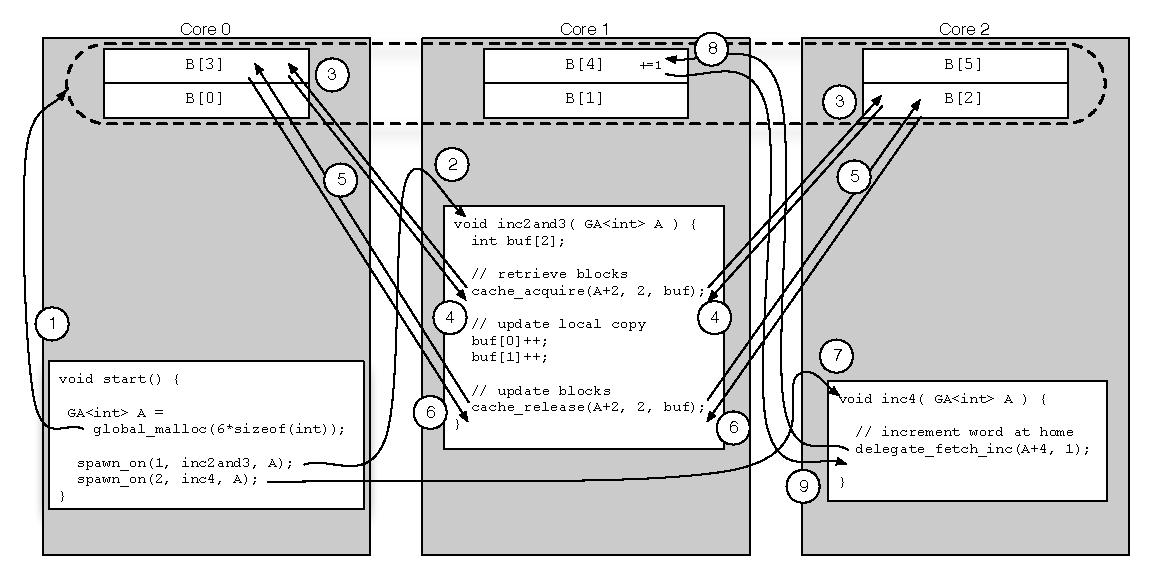
\includegraphics[width=6in]{figs/delegate-cache}
\begin{minipage}{\columnwidth}

\caption{\label{fig:delegate-cache} \textbf{Delegation and cache example:} In step 1, a core allocates an array in the global heap. It then spawns two tasks on remote cores to increment elements of the array.  The first task increments two elements of the array using cache operations. In step 2, the task is invoked. A cache request is issued for two adjacent integers starting at the second element of the array. Since these element are stored in the memories of two different cores, this requires the sending of two messages in step 3. The task is suspended until both responses arrive in step 4. The data carried in these responses is stored in the local buffer. The elements are then increment in the buffer. Then in step 5, the modified data is sent back to the home node. Acknoledgements are returned in step 6 so the task knows when the writes are complete. The second task increments an element of the array with a delegate operation. In step 7, the task is invoked. A delegate request is sent to the home core of the array element with the increment value. The task suspends until the response is received. In step 8, the increment is executed on the remote core. A response is returned in step 9 with the previous value of the array element. }

\end{minipage}
\vspace{-3ex}
\end{center}
\end{figure*}

\subsection{Communication}\label{sec:communication}

In order to mitigate the low message injection rate limits of commodity networks, Grappa's communication stack has two layers: one for user-level messages and one for network-level messages.

At the upper layer, Grappa implements asynchronous active messages \cite{vonEicken92}. Each message consists of a function pointer, an optional argument payload, and an optional data payload. When a task sends a message, the message is copied to a send queue associated with the message's destination and the task continues execution.

Grappa's lower networking layer aggregates the upper layer's messages to improve performance. Commodity networks including infiniband achieves their peak bisection bandwidth \emph{only} when the packet sizes are relatively large---on the order of multiple kilobytes. The reason for this discrepancy is the combination of overheads associated with handling each packet (in terms of bytes that form the actual packet, processing time at the card and processing on the CPU within the driver stack). Our measurements confirm manufacturers published data~\cite{infinibandbandwidth}, that with this packet size the bisection bandwidth is only a small fraction, less than 3\% of the peak bisection bandwidth.

In our experiments the vast majority of requests were smaller than 44 bytes, far too small to make efficient use of the network. To make the best use of the network, we must convert our small messages into large ones. When a task sends a message, it is not immediately sent, but rather placed in a queue specific to the destination.

There are three situations in which a queue of aggregated messages is sent. First, each queue has a message size threshold of 4096 bytes, chosen to give reasonable network performance. If the size in bytes of a queue is above the threshold, the contents of the queue are sent immediately. Second, each queue has a wait time threshold ($\approx${1ms}). If the oldest message in a queue has been waiting longer than this threshold, the contents of the queue are sent immediately, even if the queue size is lower than the message size threshold.  Third, queues may be explicitly flushed in situations where the programmer wants to minimize the latency of a message at the cost of bandwidth utilization.

The network layer is serviced by polling. Periodically when a context switch occurs, the Grappa scheduler switches to the network polling thread. This thread has three responsibilities. First, it polls the lower-level network layer to ensure it makes progress. Second, it deaggregates received messages and executes active message handlers. Third, it checks to see if any aggregation queues have messages that have been waiting longer than the threshold; if so, it sends them.

Underneath the aggregation layer, Grappa uses the \gasnet~communication library~\cite{gasnet} to actually move data. All interprocess communication, whether on or off a cluster node, is handled by the \gasnet~library. \gasnet~is able to take advantage of many communication mechanisms, including ethernet and infiniband between nodes, as well as shared memory within a node.

Some networks provide access to a remote machine's memory directly. This would seem to be a good fit for a programming model focused on global shared memory, but in fact we do not use it. In our experiments, we found that RDMA operations are subject to the same message rate limitations as all other messages on these cards, and thus using raw RDMA operations for our small messages would make inefficient use of bandwidth. Instead, we implement remote memory operations with active messages. A byproduct of this design decision is that Grappa is not limited to RDMA-capable networks.

\subsection{Performance}

To evaluate Grappa's performance with respect to the XMT, we ran each of our three benchmarks on up to 16 nodes of each machine. Grappa used 6 cores per node, with the best parameters chosen for each point. In some cases, the XMT could not run the benchmark with 2 nodes, so the point is omitted.

\begin{figure}
\begin{center}

\hspace{-1in}\begin{minipage}{0.3\textwidth}
\begin{center}
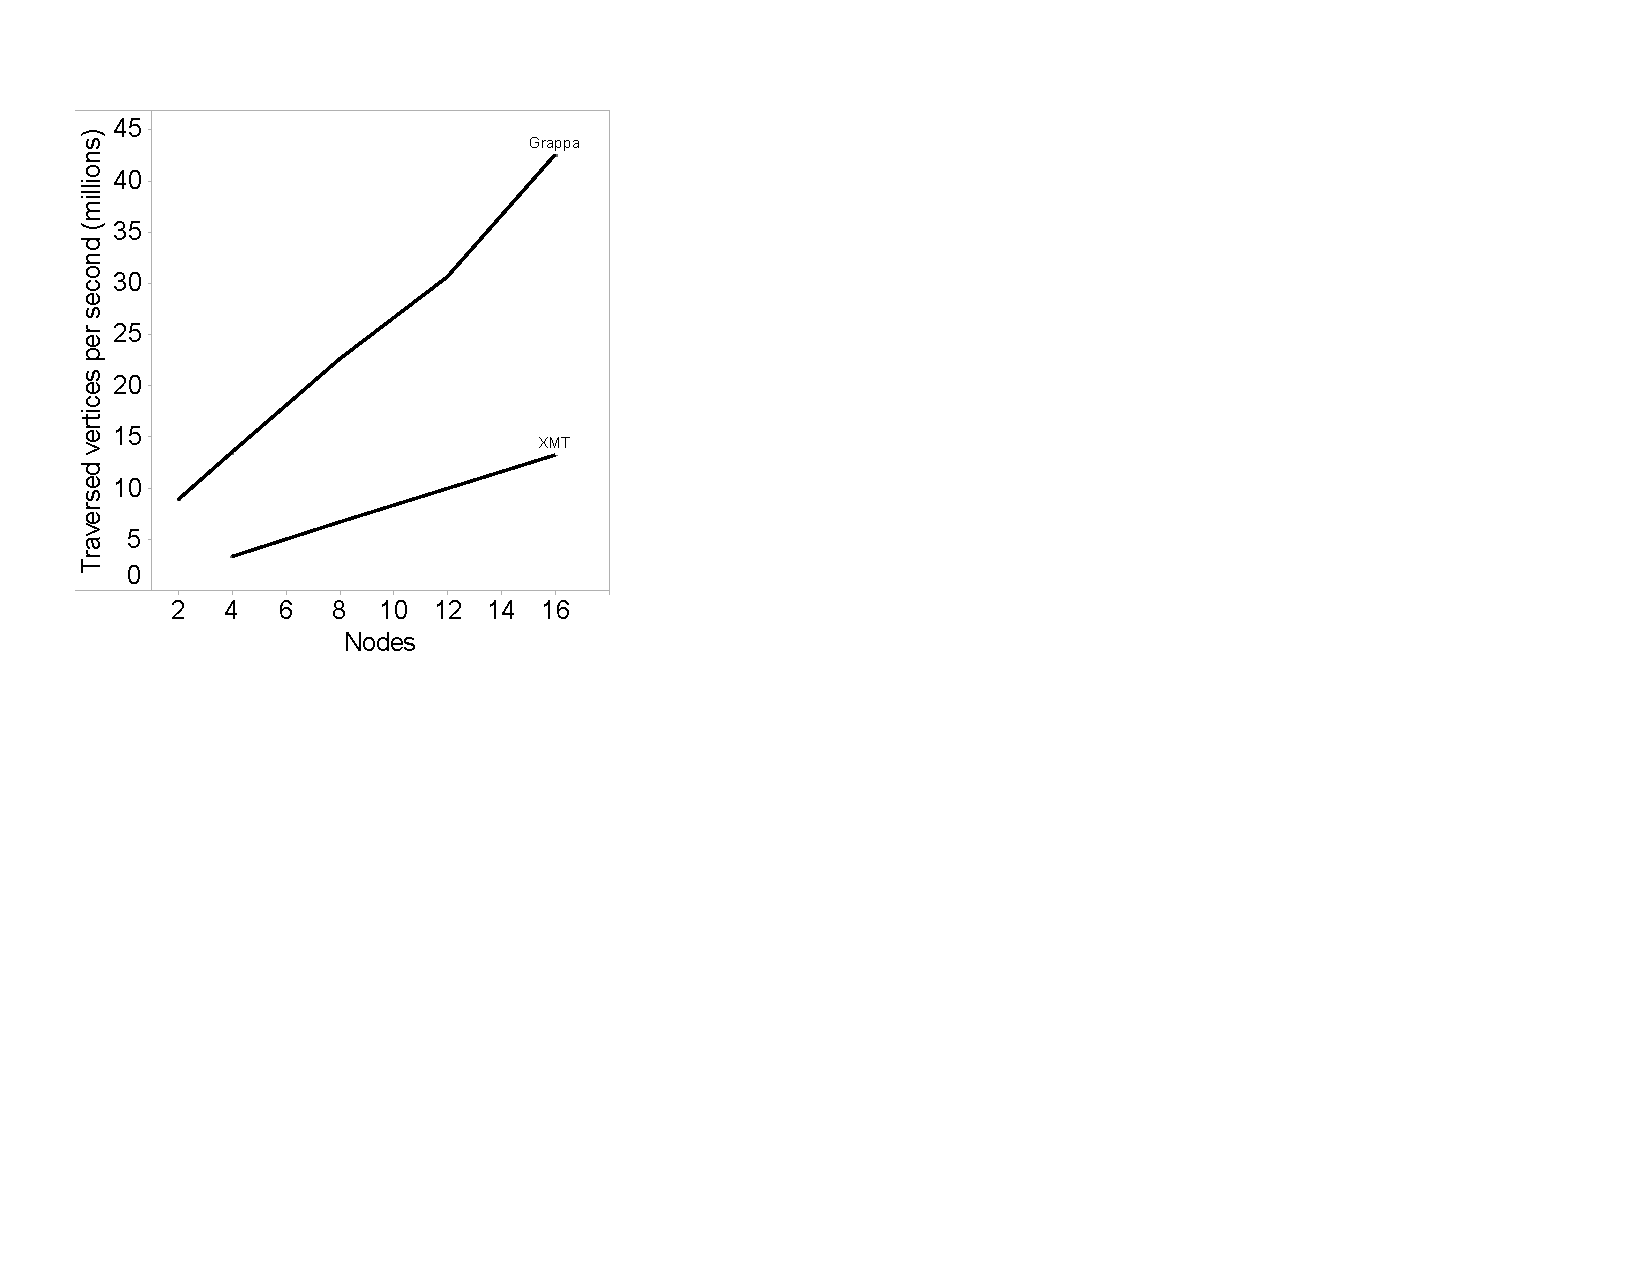
\includegraphics[width=3in]{figs/uts_performance.pdf}
\caption{\label{fig:uts_compare} Performance of in-memory unbalanced tree search.}
\end{center}
\end{minipage}
\hspace{1.25in}\
\begin{minipage}{0.3\textwidth}
\begin{center}
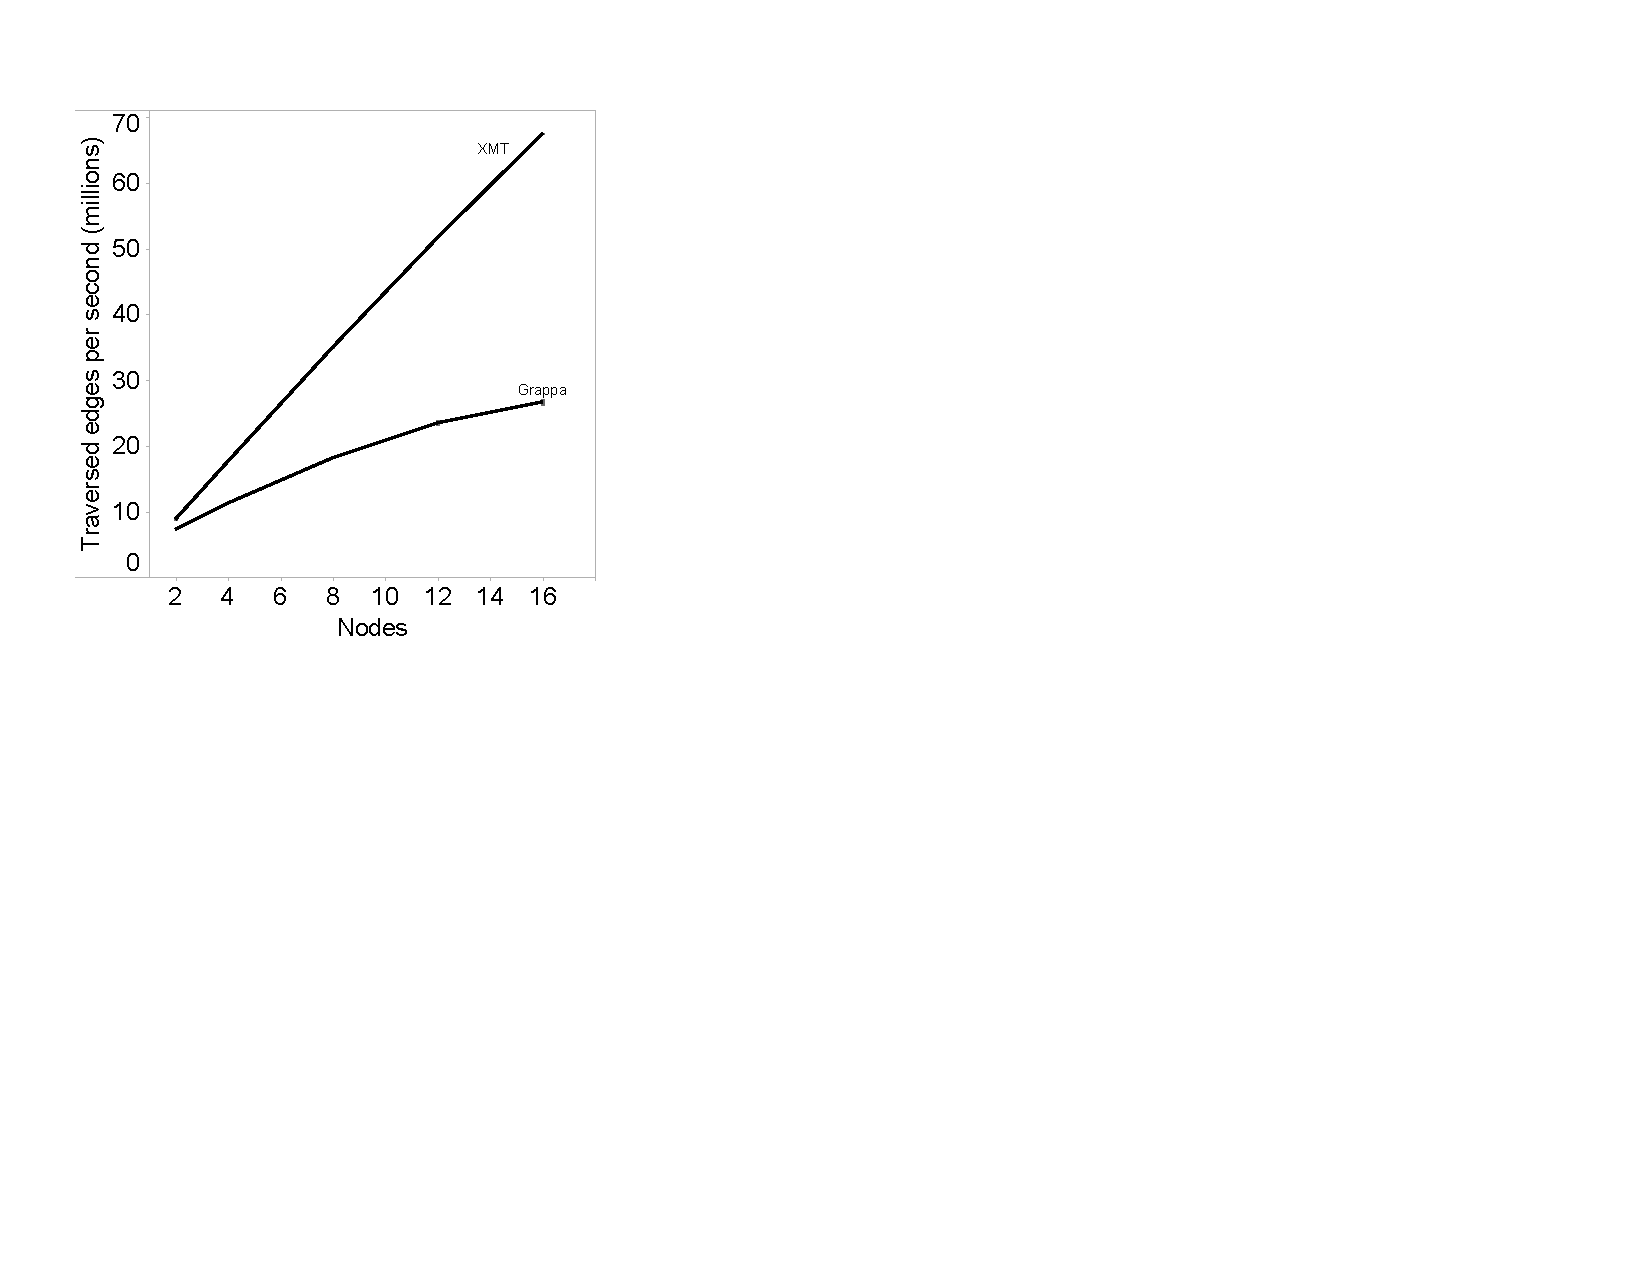
\includegraphics[width=3in]{figs/bfs_performance}
\caption{\label{fig:bfs-performance} Performance of breadth-first searcch.}
\end{center}
\end{minipage}

\end{center}
\end{figure}

\paragraph{Unbalanced tree search} We ran UTS-mem with a geometric 100M-vertex tree (T1L). Figure~\ref{fig:uts_compare} shows the performance in terms of number of vertices visited per second versus number of compute nodes. Grappa is 3.2 times faster than the XMT at 16 nodes.  As we will show later, the performance advantage Grappa has over XMT increases as more nodes are added.  The main reason Grappa performs better is the software-based delegate synchronization obviates the need for the retry-based synchronization that XMT uses.


\paragraph{BFS} We ran BFS on a synthetic Kronecker graph with $2^{25}$ vertices and $2^{29}$ edges (25 GB of data). Figure~\ref{fig:bfs-performance} shows our performance in terms of graph edges traversed per second. The XMT is 2.5 times faster than Grappa at 16 nodes.  Performance does scale at a constant rate for Grappa, suggesting that adding more nodes will increase performance.


\section{Related work}

Our efforts are built on many existing ideas in programming languages, systems and architecture. In this section we discuss related frameworks and key enabling technologies that Grappa builds upon.

\paragraph{Comparable frameworks} Distributed graph processing frameworks like Pregel~\cite{pregel:2010} and Distributed GraphLab~\cite{distgraphlab:vldb12} share similar goals as Grappa. Pregel adopts a bulk-synchronous parallel (BSP) execution model, which makes it inefficient on workloads that could prioritize vertices. GraphLab, on the other hand, schedules vertex computations individually, allowing prioritization, which gives faster convergence in a variety of iterative algorithms.  GraphLab, however, imposes a rigid computation model where programmers must express computation as transformations on a vertex and its edge list only, with information only from adjacent vertexes. Pregel is only slightly less restrictive, as the input data can be any vertex in the graph.  Grappa also supports dynamic parallelism with asynchronous execution, but parallelism is expressed as tasks or loop iterations, which is a far more general programming model for irregular computation tasks.

\paragraph{Global memory} Grappa includes a custom implementation of a software distributed shared memory (DSM) system. Many traditional software DSM systems are page based~\cite{Treadmarks,munin} and aim to hide the fact that they are built in software from applications by exploiting the processor's paging mechanisms, therefore relying heavily on locality. Instead, Grappa, like other partitioned global address space (PGAS) models, implements its DSM at the language, rather than system level. Languages such as Chapel~\cite{Chamberlain:2007}, X10~\cite{X10:2005}, and UPC~\cite{upc:2005} make accesses to shared structures look like normal memory references. As we describe later, Grappa chooses a middle ground, where global addresses are explicit in the API and local accesses are emitted conventionally by the compiler.  While Grappa's DSM system is conceptually similar to prior work, its implementation is tuned for irregular computations.  Past DSM work, being page-based, could exploit the RDMA capabilities of network hardware to move large page-sized blocks of data from node to node. In our experience, when these networks move small blocks of data (a few bytes), only a fraction of the available bandwidth is achieved. In addition, the DSM system in Grappa ends up being tightly coupled to the task scheduler in order to overlap long latency memory operations with useful computation.  For these two reasons it became necessary to build a new DSM system specifically for Grappa.

\paragraph{Multithreading} Grappa uses multithreading to tolerate memory latency. This is a well known technique. Hardware implementations include the Tera MTA~\cite{tera:mta1}, Cray XMT~\cite{feo:xmt}, Simultaneous multithreading~\cite{tullsen:smt}, MIT Alewife~\cite{agarwal:alewife}, Cyclops~\cite{almasi:cyclops}, and even GPUs~\cite{gpus}. As we describe in this paper, Grappa use a lightweight user-mode task scheduler to multiplex \emph{thousands\/} of tasks on a single processing core. The large number of tasks is required because of the extremely high internode latency Grappa is mitigating.  Grappa's task library employs several optimizations: an extremely fast task switch, a small task size, and judicious use of hardware prefetching to bring task state into the cache long before that task is actually scheduled.

\section{Proposed Research}

\subsection{Improved Networking layer}

\paragraph{Virtual topology:} Currently Grappa uses a flat network topology where each processing core in the system is individually addressed.  What this means, for example, is in a 128 node system, where each node is comprised of 16 processing cores, the network has 2048 end-points.  The aggregator treats each of these end-points individually.  This design choice is simple, and avoids lock contention within the underlying \gasnet layer, but does not scale.  As more system nodes are added, a quadratic increase in the number of threads is required in order to sustain aggregator performance.

We need to rewrite the aggregator to build in a hierarchical virtual network layer.  The first layer of this hierarchy is to treat all processors at a given system node as a single destination. We intend to continue to use the lock-free single-threaded \gasnet communication layer, as we have found the lock-based one to incur too high of an overhead for our purposes.  Thus the aggregator will need to very carefully utilize lock-free data-structures.

The second, and upper layers of the virtual topology are built from clustering system nodes into groups.  Instead of aggregating for all end-points, aggregation will occur for system nodes within a group.  A designated (and dedicated) node will act as a router, processing incoming and outgoing traffic to system nodes within the group and other groups.

Hierarchy will reduce scaling requirements from \BigO{n^2} threads to \BigO{n log(n)}.  Of course, it takes what used to be a single network hop for communication and turns it into \BigO{log(n)} hops.  More threads will be required to overcome this increased latency, but we believe only \BigO{log(n)} more, hence a real scaling benefit is achievable with the a virtual hierarchical network topology.

\paragraph{User-level RDMA:} Certain commodity networking hardware today supports remote direct memory access (RDMA).  Unfortunately, \emph{how} it is implemented is so crude that it is difficult or impossible to efficiently use in practice.  We start with a short description of the current semantics of RDMA implementations.  Next we describe the research we wish to undertake to make RDMA more useful.

Networking gear supports remote read and write operations.  Read operations take a source address and key (on a remote node), a destination address and key (on the local node), and a length.  Cards support a address translation for regions of memory that are registered with them.  These translations, indexed by the supplied key, are used to perform virtual to physical address translation.  The physical address of the destination address is similarly translated using the translation table at the local node.  Cards also support remote write operations with a similar set of semantics, where addresses are translated on cards using the cards local translation table.  Both read and write operations are asynchronous.  The requesting processor initiates the operation and then can check for completion by querying a completion queue at the local card.  \emph{Notably}, the processor(s) on the remote node are provided a polling interface whereby they can learn if a remote write operation occurred.  No such interface exists to learn about remote read or atomic operations.

This interface suffers from multiple shortcomings.  The biggest of which is that ultimately, moving data to and from a remote node constructively requires higher level semantic operations than simple reads and writes.  These higher level semantics can, of course, be synthesized from the underlying read and write primitives, but it wastes round trips and synchronization time.  One possible alternative solution is to borrow ideas from Active Messages~\cite{active-messages} and enable remote nodes to dispatch, essentially, user-level function calls.  The challenge here is to make those calls interoperate securely with a modern operating system and multicore system and be efficient.  \comment{This seems weak.  Need some more ideas here.  -Mark} 

The second challenge is the virtual to physical address translation on the cards requires the operating system to pin translations.  This removes paging flexibility from the operating system and allows user processes to (potentially unfairly) grab ahold of physical memory.  In the long run, the solution here likely lays at the intersection of what progress is occurring in virtual memory translation for I/O with virtual machines and RDMA.  Our goal will be carefully study the I/O virtualization proposals put forth by major processor manufactures and devise solutions that enable RDMA to capitalize on these developments.  \comment{weak?  -M}

The final challenge is that atomic operations via RDMA do not interact atomically with processors in a system.  Semantically it is not entire clear what happens if a processor issues an atomic operation on a memory address at the same time the network card is attempting to service a remote atomic access. \comment{maybe this is not true.  have to think some more about PCIe an what happens here.  might not be a problem.  -M}

\subsection{SSD-only data structures}

\subsection{Compiler and language support}

\subsection{Graph benchmark suite}

\newpage 
\setcounter{page}{1} 

\bibliographystyle{abbrv}
\bibliography{proposal}

\end{document}




